\chapter{Gravitazione}
Agli inizi del Cinquecento, Copernico avanzò l'ipotesi eliocentrica: il Sole, e non la Terra, era il corpo celeste attorno al quale si svolgeva il moto dei pianeti. Alla fine del secolo, le posizioni da lui assunte erano state oggetto di numerose misurazioni da parte di Brahe. Proprio su queste misure, agli inizi del Seicento, si basò Keplero per formulare le sue tre leggi.
\begin{teo}[leggi di Keplero]\hfill
    \begin{enumerate}
        \item I pianeti percorrono orbite ellittiche intorno al sole che occupa uno dei due fuochi.
        \item La velocità areale con cui il raggio vettore che unisce il Sole ad un pianeta descrive l'orbita è costante.
        \item Il quadrato del periodo di rivoluzione $T$ di ogni pianeta è proporzionale al cubo del semiasse maggiore dell'ellisse $a$, ossia $T^2=ka^3$.
    \end{enumerate}
\end{teo}
Le tre leggi di Keplero forniscono una descrizione cinematica del moto dei pianeti. La spiegazione dinamica venne trovata da Newton nel 1666 e resa nota solo nel 1687. Questa fu l'origine della Teoria della gravitazione universale.

\section{Forza gravitazionale}
Il ragionamento di Newton per determinare l'origine dinamica del moto dei pianeti, inizialmente approssimato, è il seguente. Le orbite dei pianeti, pur essendo ellittiche, sono molto prossime a circonferenze. Si supponga quindi che queste siano approssimativamente considerabili circolari. Se questo è il caso e se la velocità è costante, il moto di un pianeta è circolare uniforme. Infatti, da
\begin{equation}
    \frac{dA}{dt}=\frac{1}{2}r^2\frac{d\theta}{dt},
\end{equation}
la costanza di $dA/dt$ e $r$ implicano che $d\theta/dt$ sia costante.

La forza che agisce sul pianeta deve essere puramente centripeta in modo da permettergli di muoversi di moto circolare uniforme. Questa è
\begin{equation}
    F=m\omega^2r=m\bigg(\frac{2\pi}{T}\bigg)^2r,
\end{equation}
dove $T$ è il periodo di rivoluzione, $m$ la massa del pianeta e $r$ il raggio dell'orbita. Usando la terza legge di Keplero e confondendo $r$ con il semiasse maggiore dell'ellisse si ha
\begin{equation}
    F=\frac{4\pi^2m}{kr^2}.
\end{equation}
Quindi, la forza esercitata dal Sole sugli altri pianeti, che incurva la loro orbita, è inversamente proporzionale al quadrato della distanza dal Sole. 

Si consideri il sistema Sole-Terra. La forza agente esercitata dal Sole sulla terra è
\begin{equation}
    F_{S,T}=\frac{4\pi^2m_T}{k_Tr^2},
\end{equation}
mentre quella esercitata dalla Terra sul Sole, per il terzo principio di Newton, è
\begin{equation}
    F_{T,S}=\frac{4\pi^2m_S}{k_Sr^2}.
\end{equation}
Eguagliando queste due forze si ottiene $m_Tk_S=m_Sk_T$. Definendo la costante
\begin{equation}
    \gamma=\frac{4\pi^2}{m_Tk_S}=\frac{4\pi^2}{m_Sk_T},
\end{equation}
si ha che il modulo della forza agente tra i due corpi celesti, agente lungo la loro retta congiungente, è
\begin{equation}
    F=\gamma\frac{m_Sm_T}{r^2}.
\end{equation}
La formula ottenuta è molto semplice ed è simmetrica nei due corpi. Per questi motivi, Newton suppose che si trattasse di una legge universale ed enunciò la seguente legge.
\begin{axiom}[legge di gravitazione universale]
    Date due masse qualsiasi, di dimensioni trascurabili rispetto alla distanza mutua, tra di esse agisce una forza attrattiva diretta lungo la retta congiungente le due masse, il cui modulo dipende direttamente dal prodotto delle masse e inversamente dal quadrato della distanza.
\end{axiom}
La costante di proporzionalità $\gamma$ è una costante universale, che non dipende dai valori delle masse e dalla geometria del sistema, ma è caratteristica dell'interazione gravitazionale. In termini vettoriali, l'espressione della forza gravitazionale è
\begin{equation}
\label{eq: forza di attrazione gravitazionale}
    \vF_{1,2}=-\gamma\frac{m_1m_2}{r^2}\hatu_{1,2}.
\end{equation}
La prima verifica di questa legge è dovuta sempre a Newton. La \eqref{eq: forza di attrazione gravitazionale} deve valere anche per un corpo di massa $m$ posto sulla Terra. La forza subita dal corpo quindi è
\begin{equation}
    F=\gamma\frac{m_Tm}{r_T^2}.
\end{equation}
Questa formula è valida se si assume che un corpo a simmetrica sferica, come la Terra, eserciti una forza come se la massa fosse interamente concentrata nel suo centro. D'altra parte, la forza peso agente sul corpo è $F=mg$, per cui eguagliando le forze si ottiene
\begin{equation}
    g=\gamma\frac{m_T}{r_T^2}.
\end{equation}
Tuttavia, Newton non conosceva né il valore di $g$ né il valore di $\gamma$ né la massa della Terra $m_T$. Per risolvere il problema, Newton spostò la sua attenzione al sistema Terra-Luna. La forza esercitata dalla Terra sulla Luna è centripeta per la Luna, quindi
\begin{equation}
    F_{T,L}=\gamma\frac{m_Tm_L}{r^2_L}=m_L\omega_L^2r_L,
\end{equation}
da cui segue che $\gamma m_T=\omega_L^2r_L^3$. Pertanto, conoscendo il periodo di rotazione della Luna attorno alla Terra e la distanza Terra-Luna si può determinare il prodotto $\gamma m_T$ e quindi $g$. 

Con i valori noti oggi l'accordo è perfetto. Al tempo di Newton il valore stimato per la distanza Terra-Luna era sbagliato e solo dopo una misurazione astronomica più precisa Newton trovò un buon accordo tra $g$ e $\gamma m_T/r_T^2$. 

La misura diretta di $\gamma$, e quindi la prima determinazione della massa terrestre, venne effettuata da Cavendish nel 1798. Tramite una bilancia di torsione determinò l'attrazione gravitazionale tra due masse sferiche. Questa misura risulta molto complessa dato che l'ordine di grandezza della forza di attrazione gravitazionale è intorno ai $\SI{e-9}{\N}$. Le misure più recenti restituiscono 
\begin{equation}
    \gamma=\SI{6.67e-11}{\meter^{3}\kg^{-1}\s^{-2}},\quad m_T=\SI{5.98e24}{\kg}.
\end{equation}
\begin{obs}
    Solo conoscendo $\gamma$ si possono conoscere le masse dei corpi celesti.
\end{obs}
La \eqref{eq: forza di attrazione gravitazionale} mostra come la forza di attrazione gravitazionale sia una forza centrale. In questo modo si chiarisce la validità della seconda legge di Keplero. 

A differenza delle forze considerate in precedenza, che si manifestano al contatto (macroscopico) tra i corpi, la forza di attrazione gravitazionale si manifesta a distanza, senza che le masse vengano a contatto. In effetti, tutte le forze di interazione fondamentali sono forze a distanza, che differiscono per il raggio di azione. Altre caratteristiche importanti della forza di attrazione gravitazionale sono l'indipendenza dal moto relativo, dalla presenza di materia interposta e dallo stato di aggregazione e composizione chimica. 

\subsection{Esperimento di Cavendish}
L'esperimento di Cavendish è stato il primo esperimento volto a misurare la forza di gravità in laboratorio e il primo a ottenere valori accurati della costante gravitazionale.

L'apparecchio costruito da Cavendish prevedeva una bilancia di torsione fatta di un'asta di legno lunga tenuta sospesa da un filo, con due piccole sfere di piombo attaccate ad ogni estremità. Due sfere di piombo, molto più grandi delle altre, erano situate vicino a quelle più piccole ed erano tenute in posizione da un sistema di sospensione indipendente. L'esperimento misurò la debole attrazione gravitazionale tra le sfere piccole e quelle più grandi.

Le due sfere grandi erano posizionate sui lati opposti del braccio orizzontale di legno della bilancia. La mutua attrazione con le sfere piccole faceva ruotare il braccio, causando la torsione del filo che lo sosteneva. Il braccio cessava di ruotare dopo aver raggiunto un angolo per cui la forza di torsione del filo era bilanciata dalla forza gravitazionale combinata di attrazione tra le sfere grandi e quelle piccole. Misurando l'angolo dell'asta e conoscendo ilo momento meccanico del filo per un dato angolo, Cavendish fu in grado di determinare la forza tra le coppie di masse. Poiché la forza gravitazionale della Terra sulla sfera piccola può essere misurata direttamente pesandola, il rapporto tra le due forze permetteva di calcolare la densità della Terra utilizzando la legge di gravitazione universale.

Per ricavare la costante di gravitazione universale, si parte ricordando che, per la legge di Hooke, il momento sul filo di torsione è proporzionale all'angolo di deviazione della bilancia, in particolare $\vM_T=k\theta$, dove $k$ è il coefficiente di torsione del filo. Tuttavia, il momento può anche essere scritto come prodotto delle forze di attrazione tra le sfere e la distanza dal filo di sospensione. Poiché ci sono due coppie di sfere, ciascuna sottoposta una forza $\vF$ ad una distanza $L/2$ dall'asse della bilancia, il momento di torsione è $M_T'=LF$. Uguagliando le due formule del momento meccanico si ottiene 
\begin{equation}
    k\theta=LF.
\end{equation}
Sostituendo per $F$ il modulo di \eqref{eq: forza di attrazione gravitazionale} si ottiene
\begin{equation}
\label{eq: bilancio momenti cavendish}
    k\theta=L\frac{\gamma mM}{r^2}.
\end{equation}
L'equazione del moto dell'asta è, in modulo, $-k\theta=I\alpha$, che non è altro che l'equazione del moto armonico semplice
\begin{equation}
    \frac{d^2\theta}{dt^2}+\omega^2\theta=0,\quad\omega=\sqrt{\frac{I}{k}}.
\end{equation}
Quindi, per ricavare il coefficiente $k$, Cavendish misurò il periodo di oscillazione della bilancia di torsione dato da
\begin{equation}
    T=\frac{2\pi}{\omega}=2\pi\sqrt{\frac{I}{k}}.
\end{equation}
Trascurando la massa dell'asta di torsione stessa, il momento di inerzia della bilancia è dovuto solo alle sfere piccole
\begin{equation}
    I=m\bigg(\frac{L}{2}\bigg)^2+m\bigg(\frac{L}{2}\bigg)^2=\frac{mL^2}{2}.
\end{equation}
Sostituendo questa, il periodo di oscillazione è
\begin{equation}
    T=2\pi\sqrt{\frac{mL^2}{2k}},
\end{equation}
che risolta per $k$ restituisce
\begin{equation}
    k=2\pi^2\frac{mL^2}{T^2}.
\end{equation}
Sostituendo l'espressione ricavata per $k$ in \eqref{eq: bilancio momenti cavendish} si ottiene
\begin{equation}
    \gamma=\frac{2\pi^2Lr^2}{MT^2}\theta.
\end{equation}
Dunque, dalla conoscenza degli elementi della bilancia e dalla misura dell'angolo di deviazione $\theta$ è possibile ricavare la costante di gravitazione universale $\gamma$. 

\subsection{Massa inerziale e massa gravitazionale}
L'equazione \eqref{eq: forza di attrazione gravitazionale} esprime un particolare tipo di interazione il cui valore dalla costante $\gamma$ e dalla massa $m$ dei corpi che partecipano all'interazione. La massa $m$ in \eqref{eq: forza di attrazione gravitazionale} prende il nome di massa gravitazionale. A priori non c'è nessuna ragione che giustifichi l'uguaglianza tra la massa gravitazionale sia identica alla massa inerziale che compare nel secondo principio di Newton $\vF=m\va$. In quest'ultima, la massa $m$ caratterizza l'inerzia del corpo, qualunque sia la forza agente. Sulla superficie terrestre vale l'equazione
\begin{equation}
    m_Ig=\gamma\frac{m_{T,G}m_G}{r_T^2},
\end{equation}
dove $m_I$ e $m_G$ sono la massa inerziale e gravitazionale del corpo attratto dalla Terra, la cui massa gravitazionale è $m_{T,G}$. Si ricava
\begin{equation}
    g=\gamma\frac{m_{T,G}m_G}{r_T^2m_I}.
\end{equation}
Sperimentalmente, in uno stesso luogo $g$ è indipendente dai corpi, quindi per qualsiasi corpo il rapporto $m_G/m_I$ è pari ad una costante. Quindi, per lo meno $m_G$ e $m_I$ sono proporzionali. 

Dato che non c'è un modo diretto per misurare il rapporto $m_G/m_I$, l'ipotesi più semplice è supporre che $m_G=m_I$. Questo significa che nell'esperimento di Cavendish le masse delle sfere sono quelle inerziali e che quindi il valore di $\gamma$ si basa su questa ipotesi di uguaglianza. 

Se il rapporto $m_G/m_I$ dipendesse dai corpi, ad esempio dalla loro composizione chimica, sarebbe possibile metterlo in evidenza con il metodo seguente. \'E noto che in un sistema di riferimento terrestre (non inerziale) un filo a piombo non si dispone parallelamente alla forza di gravità, dipendente da $m_G$, in quanto risente della forza centrifuga, la quale è una forza apparente dipendente da $m_I$. Questa deviazione è piccola ma è misurabile. Quindi, due fili con appesi corpi di materiale diverso potrebbero disporsi secondo angoli diversi, se per questi il rapporto $m_G/m_I$ fosse differente. Questo metodo venne proposto alla fine dell'Ottocento da E\"otv\"os. L'esperimento non diede risultato, nel senso che il rapporto $m_G/m_I=1$ fu verificato per tutti i corpi provati entro $10^{-6}$. Le misure moderne hanno verificato l'uguaglianza entro $10^{-12}$.

\section{Campo gravitazionale}
La struttura della legge \eqref{eq: forza di attrazione gravitazionale} permette di fare la seguente considerazione. Si possono infatti scrivere
\begin{equation}
    \vF_{1,2}=\bigg(-\gamma\frac{m_1}{r^2}\hatu_{1,2}\bigg)m_2,\quad\vF_{2,1}=\bigg(-\gamma\frac{m_2}{r^2}\hatu_{2,1}\bigg)m_1
\end{equation}
e pensare che la forza gravitazionale $\vF_{1,2}$ esercitata da $m_1$ su $m_2$ sia pari al prodotto di un vettore, che non dipende da $m_2$, ma solo da $m_1$ e dalla distanza di $m_1$ da $m_2$; viceversa per $\vF_{2,1}$. 

Il vettore in questione prende il nome di campo gravitazionale, generato dalla massa sorgente del campo nel punto $P$ distante $r$ da essa. Quindi, con questa definizione si ha
\begin{equation}
\label{eq: forze di attrazione gravitazionale in termini di campo}
    \vF_{1,2}=m_2\vG_1,\quad\vF_{2,1}=m_1\vG_2.
\end{equation}
I vettori $\vG_1$ e $\vG_2$ sono diversi in modulo, ma comunque è verificato il terzo principio di Newton $\vF_{1,2}=-\vF_{2,1}$. Le formule \eqref{eq: forze di attrazione gravitazionale in termini di campo} sono valide per masse puntiformi o a simmetria sferica. In quest'ultimo caso, anche il campo è a simmetria sferica, ossia centrale, sempre rivolto verso la sorgente.

Il campo gravitazionale totale $\vG$ in un punto $P$, generato da un numero $n$ di masse puntiformi $m_1,\dots,m_n$, si ottiene sommando vettorialmente i vari contributi delle singole masse, quindi
\begin{equation}
    \vG=\sum_{i=1}^n\vG_i=\sum_{i=1}^n-\gamma\frac{m_i}{r_i^2}\,\hatu_i.
\end{equation}
Il campo gravitazionale $\vG$ in un punto $P$ dovuto ad una massa $m$ continua contenuta in una regione limitata si calcola dividendo $m$ in parti infinitesime $dm$, ognuna generante una campo $d\vG$ in $P$ che vale
\begin{equation}
    d\vG=-\gamma\frac{dm}{r^2}\hatu,
\end{equation}
e integrando vettorialmente su tutti i contributi si ha
\begin{equation}
    \vG(P)=\int_V-\gamma\frac{dm}{r^2}\hatu=\int_V-\gamma\rho\frac{dV}{r^2}\hatu.
\end{equation}
La forza tra due corpi estesi $C_1$ e $C_2$ di masse $m_1$ e $m_2$ si ottiene calcolando in ciascun elemento di $m_2$ la forza $d\vF_{1,2}=dm_2\vG_1$, esercitata dal corpo di massa $m_1$, e integrando vettorialmente su tutto $C_2$, ovvero
\begin{equation}
    \vF_{1,2}=\int_{C_2}\vG_1\,dm_2.
\end{equation}
\begin{obs}
    La nozione di campo gravitazionale è indipendente dalle masse $m_1$ e $m_2$? Se si supponesse di rimuovere la massa $m_2$, il campo gravitazionale generato da $m_1$ continua ad esistere in quanto modifica lo spazio circostante indipendente dalla presenza di corpi su cui può agire, in accordo con le previsioni della Relatività generale. Se invece si supponesse di rimuovere la sorgente del campo gravitazionale, allora il campo effettivamente cessa di esistere. Tuttavia, un caso particolare è quando la massa che genera tale campo è molto lontana da dove viene rivelato. Ad esempio, una stella molto lontana dalla Terra che genera un campo gravitazionale molto inteso, potrebbe cessare di esistere, a seguito di una supernova, ma suo il campo gravitazionale prima di smettere di essere rivelato sulla Terra, deve prima percorre la distanza che lo separa da essa. Quindi, anche se la sorgente del campo non esiste più, il suo effetto può ancora essere rivelato per un certo periodo di tempo. Il campo gravitazionale si propaga sotto forma di onde gravitazionali, rivelate per la prima volta nel 2015 dall'interferometro LIGO. 
\end{obs}

\section{Energia e potenziale gravitazionale}
La forza gravitazionale è conservativa. L'affermazione è già noto sia vera in quanto è una forza centrale, tuttavia il calcolo esplicito permette di determinare la forma del potenziale gravitazionale. 

Si consideri una massa $m_2$ sottoposta al campo gravitazionale generato da una massa $m_1$. Il lavoro compiuto durante uno spostamento $d\vs$ di $m_2$ è
\begin{equation}
    dW=\vF\cdot d\vs=-\gamma\frac{m_1m_2}{r^2}\hatu_1\cdot d\vs.
\end{equation}
Il prodotto scalare $\hatu_1\cdot d\vs$ è pari alla proiezione di $d\vs$ su $\hatu_1$, quindi è pari a $dr$, ossia alla variazione del modulo della distanza tra le due masse a seguito dello spostamento. Quindi, integrando l'espressione di $dW$ si ottiene
\begin{equation}
    \begin{split}
        W=\int_A^BdW=\int_{r_A}^{r_B}-\gamma\frac{m_1m_2}{r^2}\,dr=-\gamma\frac{m_1m_2}{r_A}-\bigg(-\gamma\frac{m_1m_2}{r_B}\bigg)=-\Delta U_{AB}.
    \end{split}
\end{equation}
Quindi, come previsto, il lavoro della forza gravitazionale non dipende dalla traiettoria e può essere espresso in termini di una funzione di stato $U(r)$, che prende il norme di energia potenziale gravitazionale, definita da
\begin{equation}
\label{eq: energia potenziale gravitazionale}
    U(r)=-\gamma\frac{m_1m_2}{r}.
\end{equation}
\begin{obs}
    A rigore $U(r)$ è definita a meno di una costante additiva $C$. Tuttavia, è ragionevole pensare che a distanza infinita l'energia potenziale gravitazionale tenda a zero. In tal caso, la costante, che ha il significato di valore dell'energia potenziale per $r=\infty$, si annulla. Infatti
    \begin{equation}
        U(r\to\infty)=-\gamma\frac{m_1m_2}{r}+C=0\Rightarrow C=0.
    \end{equation}
\end{obs}
Quando $m_2$ si avvicina a $m_1$, la forza gravitazionale compie un lavoro positivo e $m_2$ acquista energia cinetica. Dato che la forza è conservativa, l'energia meccanica si deve conservare. Quindi, se l'energia cinetica di $m_2$ aumenta, la sua energia potenziale deve diminuire. Essendo nulla per distanze infinite, $U(r)$ deve essere negativa per distanze finite.  

Anche all'energia potenziale gravitazionale può essere associato un potenziale. In questo caso, $U(r)$ si può scrivere come $U(r)=m_2V_1(r)$, dove $V(r)$ prende il nome di potenziale gravitazionale generato da $m_1$ ed è dato da
\begin{equation}
\label{eq: potenziale gravitazionale}
    V_1(r)=-\gamma\frac{m_1}{r}.
\end{equation}
La situazione è simmetrica nelle masse, infatti si può anche scrivere 
\begin{equation}
    U(r)=m_1V_2(r),\quad V_2(r)=-\gamma\frac{m_2}{r}.
\end{equation}
Il lavoro per uno spostamento generico della massa $m_2$ dalla posizione $A$ alla posizione $B$ nel campo $m_1$ è
\begin{equation}
    W=-\Delta U_{AB}=-m_2\Delta V_1=m_2[V_1(r_B)-V_1(r_A)].
\end{equation}
Tra il campo e il potenziale gravitazionale esiste la relazione fondamentale
\begin{equation}
    \vG=-\nabla V.
\end{equation}
Come visto per il campo gravitazionale, anche il potenziale generato da un numero $n$ di masse si ricava calcolando la somma dei singoli contributi finiti, o infinitesimi nel caso di corpi estesi. Tuttavia, nel caso del potenziale la somma è scalare non vettoriale, risultando più semplice dal punto di vista analitico. 
\begin{figure}[h]
    \centering
    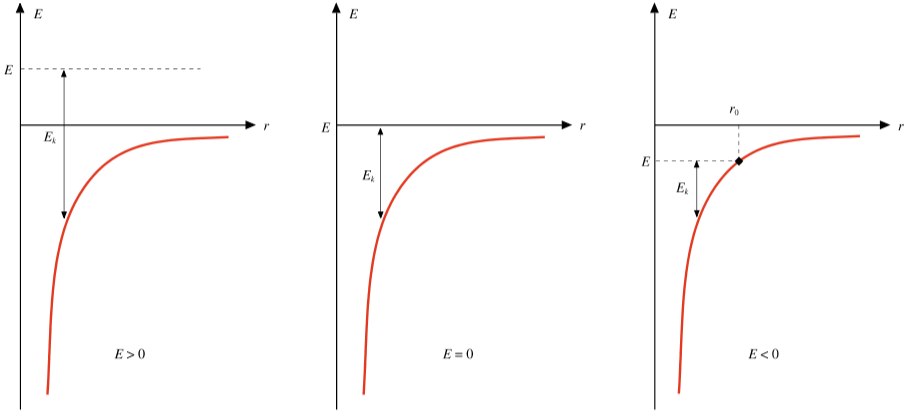
\includegraphics[width=0.9\linewidth]{Immagini/energia orbite.png}
    \caption{confronto tra energia meccanica, potenziale e cinetica per le diverse orbite.}
    \label{fig: energie orbite}
\end{figure}

L'energia totale di un sistema a due masse può assumere valore positivo, nullo o negativo a seconda che sia verificata una delle condizioni
\begin{equation}
    K>|U|,\quad K=|U|,\quad K<|U|.
\end{equation}
Nei grafici in figura \ref{fig: energie orbite} sono rappresentati i tre casi: $r$ è la distanza mutua, $E$ è l'energia totale costante, la doppia freccia indica la differenza $E-U=K$ per un particolare valore di $r$, mentre la curva continua mostra $U=-\gamma m_1m_2/r$ ed è la stessa nei tre casi. Nei primi due casi non ci sono limiti, mentre nel terzo $r$ è limitato da $r\le r_0$, altrimenti si avrebbe $K>E$. Queste considerazioni vengono parzialmente corrette a seguito del calcolo esplicito per l'energia totale del sistema di due masse, valida anche per orbite non circolari. In particolare, si otterrà che se $E>0$ l'orbita è iperbolica, se $E=0$ l'orbita è parabolica, mentre se $E<0$ l'orbita è ellittica. Le traiettorie ellittiche possono essere di tre diverse, di cui una in realtà circolare. 

\section{Teorema di Gauss per \texorpdfstring{$\vG$}{G} e distribuzioni sferiche}
Si consideri un certo numero di masse e una superficie geometrica chiusa che ne racchiude $n$. In ogni punto della superficie si determina $\vG$, che è dovuto a tutte le masse presenti, sia interne che esterne, e si calcola la quantità scalare
\begin{equation}
    d\Phi=\vG\cdot\hatu_N\,dS,
\end{equation}
dove $\hatu_N$ è il vettore normale alla superficie, che si assume essere orientato verso l'esterno, e $dS$ è l'elemento di superficie intorno al quale è calcolato $\vG$. L'integrale esteso a tutta la superficie restituisce 
\begin{equation}
    \Phi=\oint d\Phi=\oint\vG\cdot\hatu_N\,dS,
\end{equation}
che prende il nome di flusso del campo gravitazionale attraverso la superficie $S$. A questo punto è fondamentale il seguente teorema.
\begin{teo}[teorema di Gauss]
    Il flusso del campo gravitazionale attraverso una superficie chiusa è proporzionale alla somma delle masse interne alla superficie secondo
    \begin{equation}
        \Phi=-4\pi\gamma\sum_{i=1}^nm_i.
    \end{equation}
\end{teo}
\begin{proof}
    Il differenziale del flusso di campo gravitazionale è
    \begin{equation}
        d\Phi=\vG\cdot\hatu_N\,dS=-\gamma\frac{m}{r^2}(\hatu_r\cdot\hatu_N)\,dS=-\gamma\frac{m}{r^2}\,dS,
    \end{equation}
    dove il differenziale $dS$ corrisponde ad una porzione infinitesima di superficie sferica che, in coordinate sferiche, è data da
    \begin{equation}
        dS=r^2\sin{\theta}\,d\theta d\phi.
    \end{equation}
    Quindi integrando il differenziale $d\Phi$, in cui si è sostituito $dS$, si ottiene
    \begin{equation}
        \Phi=\int d\Phi=-\gamma\frac{m}{r^2}r^2\int_0^{\pi}\sin{\theta}\,d\theta\int_0^{2\pi}d\phi=-4\pi\gamma m.
    \end{equation}
    La dimostrazione è analoga nel caso in cui il campo gravitazione sia $\vG=\nsum_i\vG_i$ e la massa compresa all'interno della superficie di Gauss sia $m=\nsum_im_i$. 
\end{proof}
Il teorema permette di verificare che il campo generato da una distribuzione sferica di massa è uguale a quello generato da una massa puntiforme identica posta nel centro della distribuzione. Si consideri quindi una distribuzione sferica superficiale uniforme di massa $m$ di raggio $R$. Nel punto $P$, esterno alla distribuzione, il campo $\vG$ è radiale ed è dovuto alla somma di contributi simmetrici, se così non fosse la distribuzione non sarebbe uniforme. In qualsiasi altro punto che abbia la stessa distanza $r$ di $P$ dal centro della distribuzione il campo ha lo stesso valore, in quanto dipende solo dal modulo di $r$, ossia è radiale $\vG=G(r)\hatu_r$. Per calcolare $G(r)$ si considera come superficie di integrazione una seconda superficie sferica $S$ concentrica alla distribuzione di raggio $r\ge R$. In tal caso, si ha che il flusso attraverso $S$ è
\begin{equation}
    \Phi=\oint-G(r)\hatu_r\cdot\hatu_N\,dS=G(r)\oint dS=4\pi r^2G(r).
\end{equation}
Dato che per il teorema di Gauss $\Phi=4\pi\gamma m$, uguagliando le due espressione del flusso si ottiene
\begin{equation}
    G(r)=\gamma\frac{m}{r^2},
\end{equation}
come se $m$ fosse concentrata nel centro della distribuzione di massa. Il risultato vale per $r\ge R$, invece all'interno, per $r<R$, qualsiasi superficie di integrazione si consideri non contiene alcuna massa e quindi il flusso attraverso essa è nullo, in altre parole $G=0$ per $r<R$.

Se $m$ è distribuita uniformemente in tutto il volume sferico, all'esterno l'espressione di $G(r)$ è la medesima, mentre per $r<R$ il valore non è più nullo. Sfruttando la simmetria radiale, all'interno di una superficie sferica $S_1$ di raggio $r\le R$ la massa contenuta $m(r)$ è minore di $m$. Dato che la distribuzione è uniforme, il rapporto tra $m(r)$ e $m$ è uguale al rapporto tra i volumi occupati, ovvero a $r^3/R^3$, per cui
\begin{equation}
    m(r)=\frac{mr^3}{R^3}.
\end{equation}
Sostituendo questa nell'espressione di $\Phi$ e usando il teorema di Gauss si ha
\begin{equation}
    \Phi(r)=4\pi r^2G(r)=4\pi\gamma m(r)=4\pi\gamma m\frac{r^3}{R^3},
\end{equation}
da cui
\begin{equation}
    G(r)=\gamma\frac{m}{R^3}r.
\end{equation}
Riassumendo, l'intensità del campo gravitazionale in funzione della distanza $r$ dal centro della distribuzione volumica sferica omogenea di massa $m$ è
\begin{equation}
\label{eq: campo gravitazionale in funzione di r}
    G(r)=\begin{cases}
        \gamma\dfrac{m}{r^2},\quad r\ge R\\[1.5ex]
        \gamma\dfrac{m}{R^3}r,\quad r<R
    \end{cases}.
\end{equation}
\begin{obs}
    Considerando una massa puntiforme $m_p$, da \eqref{eq: campo gravitazionale in funzione di r} si ha che la forza subita da $m_p$ è
    \begin{equation}
        \vF=m_p\vG=-\gamma\frac{m_pm}{R^3}r\hatu_r=-K\vr,
    \end{equation}
    ossia è una forza di tipo elastico. Se lungo un diametro della distribuzione si creasse un foro e si lasciasse cadere la massa $m_p$ all'interno di esso, questa si muoverebbe di moto armonico con ampiezza pari al raggio $R$ della distribuzione. 
\end{obs}
Dato che l'espressione di $G(r)$ per distanze maggiori del raggio della distribuzione sferica è sempre la stessa, si può dimostrare che la forza gravitazionale tra due sfere omogenee di masse $m_1$ e $m_2$, poste ad una distanza $r$ tra i loro centri $O_1$ e $O_2$, è uguale alla forza gravitazionale tra due masse puntiformi $m_1$ e $m_2$ distanti $r$.

Ciascun elemento $dm_2$ della seconda sfera è soggetto ad una forza gravitazionale equivalente a quella generata da una massa puntiforme $m_1$ posta in $O_1$. Quindi, dalla definizione di $\vG$ e di forza di attrazione gravitazionale si ha
\begin{equation}
    d\vF_{1,2}=dm_2\vG_1=-\gamma\frac{m_1 dm_2}{r_1^2}\hatu_1.
\end{equation}
Per calcolare la risultante di tutte queste forze $d\vF_{1,2}$ si osserva che, il base al terzo principio di Newton, $dm_2$ esercita in $O_1$ una forza uguale e opposta
\begin{equation}
    d\vF_{2,1}=-d\vF_{1,2}=\gamma\frac{m_1 dm_2}{r_1^2}\hatu_1,
\end{equation}
e che l'effetto risultante in $O_1$ è quello di una massa puntiforme $m_2$ posta in $O_2$. Quindi, la forza risultante, in modulo, è
\begin{equation}
    F=\gamma\frac{m_1m_2}{r^2}.
\end{equation}
Il risultato è vero anche se i raggi delle due sfere sono confrontabili con la distanza tra i due centri o anche se le sfere sono a contatto. Si può anche lasciare l'ipotesi che la distribuzione delle masse sia omogenea, in quanto è sufficiente che tale distribuzione vari unicamente in funzione della distanza dal centro in modo da conservare la simmetrica sferica.
\begin{obs}
    Queste proprietà sono tutte derivate dal teorema di Gauss e quindi valgono per tutti i campi proporzionali a $1/r^2$, compreso il campo elettrostatico. 
\end{obs}

\subsection{Energia gravitazionale di una sfera omogenea}
Si supponga di costruire una sfera di massa $m$ e raggio $R$ per gusci successivi, ognuno compreso tra $r$ e $r+dr$. Il lavoro per portare da distanza infinita a distanza $r$ dal centro la massa $dm$ che si distribuisce nel guscio tra $r$ ed $r+dr$ è
\begin{equation}
    dW=-dU=\gamma\frac{m(r)dm}{r}.
\end{equation}
Sapendo che $m(r)=mr^3/R^3$, si ha
\begin{equation}
    dm=\frac{m}{R^3}d(r^3)=\frac{3mr^2}{R^3}dr.
\end{equation}
Pertanto
\begin{equation}
    dW=3\gamma\frac{m^2}{R^6}r^4\,dr,
\end{equation}
la quale integrata tra $0$ ed $R$ restituisce il lavoro necessario per costruire l'intera sfera
\begin{equation}
    W=\frac{3}{5}\gamma\frac{m^2}{R}.
\end{equation}
Il lavoro è fornito dalla forza gravitazionale ed è uguale a $U_i-U_f$. Però, $U_i=0$ in quanto inizialmente tutte le parti della sfera sono infinitamente lontane tra di loro, quindi
\begin{equation}
    U_f=-W=-\frac{3}{5}\gamma\frac{m^2}{R}.
\end{equation}

\subsection{Velocità di fuga e orbita circolare}
La velocità di fuga è la velocità minima necessaria affinché un oggetto possa sfuggire all'attrazione gravitazionale di un corpo celeste senza ulteriore apporto di energia. Si parte dall'uguaglianza tra l'energia cinetica iniziale dell'oggetto e l'energia potenziale gravitazionale necessaria per allontanarlo indefinitamente. L'energia cinetica di $m$ è data dall'espressione $mv^2/2$, mentre l'energia potenziale gravitazionale in prossimità della superficie del pianeta di massa $M$ è $-\gamma m M/R_T$. Affinché l'oggetto possa allontanarsi indefinitamente, la sua energia meccanica totale deve essere nulla, ovvero
\begin{equation}
    \frac{1}{2}mv^2-\gamma\frac{mM}{R_T} = 0.
\end{equation}
Risolvendo rispetto a $v$, si ottiene l'espressione della velocità di fuga:
\begin{equation}
    v = \sqrt{\frac{2 \gamma M}{R_T}}.
\end{equation}
Un altro aspetto importante riguarda l'energia potenziale di un oggetto in orbita a una distanza $R_T+h$ dal centro del pianeta. In questo caso, l'energia potenziale gravitazionale è data da
\begin{equation}
    U(R_T + h) = -\gamma\frac{mM}{R_T + h}.
\end{equation}
Nel caso in cui $h\ll R_T$, si può espandere l'espressione tramite l'approssimazione
\begin{equation}
    \frac{1}{R_T + h} \approx \frac{1}{R_T} \left( 1 - \frac{h}{R_T} \right).
\end{equation}
Pertanto, l'energia potenziale può essere riscritta come
\begin{equation}
    U(R_T + h) \approx -\frac{\gamma m M}{R_T} + \frac{\gamma m M}{R_T^2} h.
\end{equation}
Ricordando che $g=\gamma M/R_T^2$ e notando che il termine $-\gamma m M/R_T$ è una costante, l'energia potenziale $U$ si può scrivere come
\begin{equation}
    U(R_T+h)=mgh+costante.
\end{equation}
Quindi, ridefinendo in modo opportuno la costante è possibile scrivere l'energia potenziale gravitazionale $U$ rispetto alla superficie terrestre come $mgh$. 

\section{Moto dei pianeti}
L'obiettivo è ora dimostrare che le orbite dei pianeti sono ellittiche e che il quadrato del periodo di rivoluzione è proporzionale al cubo del semiasse maggiore, ossia si vogliono dimostrare la prima e la terza legge di Keplero. 

Si considerino due masse isolate $m$ ed $M$, che possono essere indifferentemente puntiformi o estese, tra le quali agisca una forza gravitazionale $\vF=\gamma mM/r^2$. In un sistema di riferimento inerziale 
\begin{equation}
    \vF=m\va_m,\quad\vF=M\va_M.
\end{equation}
L'accelerazione relativa di $m$ rispetto ad $M$ è
\begin{equation}
    \va=\va_m-\va_M=\bigg(\frac{1}{m}+\frac{1}{M}\bigg)\vF=\frac{\vF}{\mu},
\end{equation}
dove $\mu=mM/(m+M)$ è detta massa ridotta del sistema. Pertanto, $\vF=\mu\va$. Quindi, il moto relativo di due punti materiali sottoposti alla loro interazione mutua è equivalente al moto di un punto con massa uguale alla massa ridotta e sottoposto ad una forza uguale a quella di interazione mutua. In altre parole, l'equazione del moto di $m$ rispetto ad $M$, $\vF=\mu\va$, è identica a quella valida in un sistema di riferimento inerziale in cui $M$ è fissa, con il solo scambio $m\to\mu$ e con la forza $\vF$ immutata, anche se $M$ si muove di moto accelerato. Il risultato non dipende dal tipo di forza agente e mostra che il problema del moto relativo di due punti materiali può sempre essere ricondotto a quello di un unico punto. In questo caso, l'equazione del moto è
\begin{equation}
\label{eq: eqzn. moto dei pianeti}
    -\gamma\frac{mM}{r^2}\hatu_r=\mu a_r\hatu_r,
\end{equation}
dove $a_r$ è il modulo dell'accelerazione radiale.

Dato che si sta studiando un sistema isolato di due punti che interagiscono tra di loro tramite la forza di attrazione gravitazionale, che è una forza conservativa, allora valgono la conservazione della quantità di moto totale $\vp$, che implica la velocità del centro di massa $\vcm$ costante, la conservazione del momento angolare $\vL$ e la conservazione dell'energia meccanica $E$. Il fatto che $\vL=\vr\times\vp$ è costante, implica che il moto si svolge sul piano identificato dai vettori $\vr$ e $\vp$. Per descrivere il moto si usano le coordinate polari, in tal caso la velocità ha la forma
\begin{equation}
    \vv=\frac{dr}{dt}\hatu_r+r\frac{d\theta}{dt}\hatu_\theta.
\end{equation}
L'energia meccanica è data da
\begin{equation}
    \begin{split}
        E&=\frac{1}{2}\mu(\vv\cdot\vv)-\gamma\frac{mM}{r} \\
        &=\frac{1}{2}\mu\bigg(\frac{dr}{dt}\bigg)^2+\frac{1}{2}\mu r^2\bigg(\frac{d\theta}{dt}\bigg)^2-\gamma\frac{mM}{r} \\
        &=\frac{1}{2}\mu\bigg(\frac{dr}{dt}\bigg)^2+\frac{1}{2}\mu\frac{L^2}{r^2\mu^2}-\gamma\frac{mM}{r} \\
        &=\frac{1}{2}\mu\bigg(\frac{dr}{dt}\bigg)^2+\frac{L^2}{2\mu r^2}-\gamma\frac{mM}{r},
    \end{split}
\end{equation}
dove si è usata la relazione
\begin{equation}
    L=\mu r^2\frac{d\theta}{dt}\Rightarrow\frac{L}{\mu}=r^2\frac{d\theta}{dt}.
\end{equation}
Dato che gli ultimi due addendi dipendono solo da $r$, si introduce il potenziale efficace
\begin{equation}
    U_{eff}(r)=\frac{L^2}{2\mu r^2}-\gamma\frac{mM}{r}.
\end{equation}
Quindi, l'energia meccanica è
\begin{equation}
    E=\frac{1}{2}\mu\bigg(\frac{dr}{dt}\bigg)^2+U_{eff}(r).
\end{equation}
Osservando la forma del potenziale efficace, si nota che per piccoli valori di $r$ il termine dominante è il primo, proporzionale ad $1/r^2$, mentre per grandi valori di $r$ il termine dominante è il secondo, proporzionale ad $1/r$. Il grafico del potenziale efficace in funzione di $r$ è mostrato nella figura \ref{fig: potenziale efficace}.
\begin{figure}[h]
    \centering
    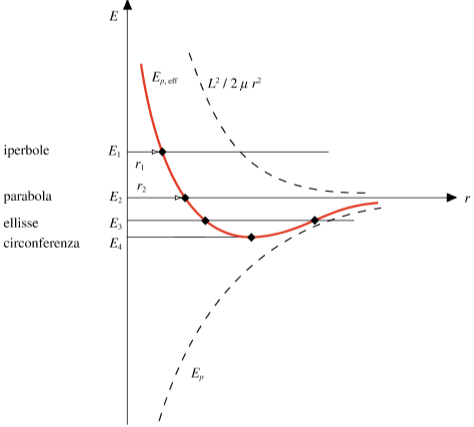
\includegraphics[width=0.6\linewidth]{Immagini/potenziale efficace.png}
    \caption{andamento del potenziale efficace in funzione della distanza tra $m$ ed $M$.}
    \label{fig: potenziale efficace}
\end{figure}


\paragraph{Proprietà delle coniche.} Prima di studiare ulteriormente il moto dei pianeti, è necessario introdurre alcune proprietà delle coniche. Prima di tutto, una conica è definita come il luogo dei punti per i quali il rapporto tra la distanza da un punto, detto fuoco, e la distanza da una retta, detta direttrice, è pari ad una costante positiva $\epsilon$ che prende il nome di eccentricità ed è data da
\begin{equation}
\label{eq: defn. eccentricità}
    \epsilon=\frac{\overline{PF}}{\overline{PQ}}=\frac{r}{r+d\cos\theta},
\end{equation}
dove $d$ è la distanza tra il fuoco e la direttrice, un parametro noto. In coordinate polari, partendo da \eqref{eq: defn. eccentricità}, l'equazione delle conica di centro $F$ è
\begin{equation}
\label{eq: eqzn. coniche}
    \frac{1}{r}=\frac{1}{\epsilon d}-\frac{\cos\theta}{d}.
\end{equation}
La conica può essere un'ellisse se $\epsilon<1$, una parabola se $\epsilon=1$, un'iperbole se $\epsilon>1$, oppure degenera in una circonferenza se $\epsilon=0$. In particolare, per un'ellisse di semiassi $a$ e $b$ valgono le relazioni
\begin{equation}
\label{eq: relazioni ellisse}
    a=\frac{\epsilon d}{1-\epsilon^2},\quad b=a\sqrt{1-\epsilon^2},\quad\epsilon^2=1-\frac{b^2}{a^2},\quad A=\pi a^2\sqrt{1-\epsilon^2}.
\end{equation}

Per esprimere l'accelerazione radiale $\va_r$ in \eqref{eq: eqzn. moto dei pianeti} si può usare la formula di Binet
\begin{equation}
    \va_r=-\frac{L^2}{\mu^2r^2}\bigg[\frac{d^2}{d\theta^2}\bigg(\frac{1}{r}\bigg)+\frac{1}{r}\bigg]\hatu_r.
\end{equation}
Sostituendola in \eqref{eq: eqzn. moto dei pianeti} e considerando i moduli si ottiene
\begin{equation}
    -\gamma\frac{mM}{r^2}=-\mu\frac{L^2}{\mu^2r^2}\bigg[\frac{d^2}{d\theta^2}\bigg(\frac{1}{r}\bigg)+\frac{1}{r}\bigg],
\end{equation}
da cui si trova l'equazione differenziale
\begin{equation}
    \frac{d^2}{d\theta^2}\bigg(\frac{1}{r}\bigg)+\frac{1}{r}=\gamma\mu\frac{mM}{L^2},
\end{equation}
la cui soluzione è la funzione $r(\theta)$ che corrisponde alla traiettoria di $m$ rispetto ad $M$ in coordinate polari. A primo membro si può riconoscere la struttura dell'equazione del moto armonico semplice con un termine aggiuntivo che la rende non omogenea. La soluzione generale di questa equazione è $A\cos\theta+S_p$, dove $S_p$ è una soluzione particolare dell'equazione di partenza. Una soluzione particolare è uguale al termine che compare a secondo membro, ossia $S_p=\gamma\mu mM/L^2$. Pertanto, la soluzione dell'equazione differenziale è
\begin{equation}
\label{eq: soluzione eq. diff.}
    \frac{1}{r}=\gamma\mu \frac{mM}{L^2}+A\cos{\theta},  
\end{equation}
che ha la stessa forma dell'equazione delle coniche \eqref{eq: eqzn. coniche}. Pertanto, la traiettoria è una conica. Dal confronto di \eqref{eq: soluzione eq. diff.} con \eqref{eq: eqzn. coniche} si ottiene che
\begin{equation}
    L^2=\gamma\mu mM\epsilon d.
\end{equation}
Quindi, i parametri della traiettoria $\epsilon$ e $d$ stabiliscono il valore costante del momento angolare della massa $m$. 

L'energia meccanica di $m$ è la somma dell'energia cinetica e dell'energia potenziale
\begin{equation}
    E=\frac{1}{2}\mu\bigg(\frac{dr}{dt}\bigg)^2+\frac{1}{2}\mu r^2\bigg(\frac{d\theta}{dt}\bigg)^2-\gamma\frac{mM}{r}. 
\end{equation}
I termini che compaiono a secondo membro di questa equazione possono essere riscritti come segue. Per il primo membro si riprende l'equazione \eqref{eq: eqzn. coniche} e ne si prende la derivata, ottenendo
\begin{equation}
    \frac{d}{dt}\bigg(\frac{1}{r}\bigg)=\frac{d}{dt}\bigg(\frac{1}{\epsilon d}-\frac{\cos\theta}{d}\bigg)\Rightarrow\frac{dr}{dt}=-\frac{r^2\sin\theta}{d}\frac{d\theta}{dt}.
\end{equation}
Per il secondo termine, dato che la forza gravitazionale è una forza centrale si può usare 
\begin{equation}
    L=\mu r^2\frac{d\theta}{dt},
\end{equation}
in modo da poter scrivere che
\begin{equation}
    \frac{1}{2}\mu r^2\bigg(\frac{d\theta}{dt}\bigg)^2=\frac{1}{2}\frac{L^2}{\mu r^2}.
\end{equation}
Infine, per il terzo termine usando che $L^2=\gamma\mu mM\epsilon d$ si ha che
\begin{equation}
    -\gamma\frac{mM}{r}=-\frac{L^2}{\epsilon d\mu r}.
\end{equation}
Mettendo insieme questi risultati si ha che l'energia meccanica è
\begin{equation}
    E=\frac{1}{2}\frac{\sin^2\theta}{d^2}\frac{L^2}{\mu}+\frac{1}{2}\frac{L^2}{\mu r^2}-\frac{L^2}{\epsilon d\mu r}.
\end{equation}
Utilizzando l'equazione \eqref{eq: eqzn. coniche} per riscrivere $1/r$ ed $1/r^2$, insieme alla relazione $L^2=\gamma\mu mM\epsilon d$, si ottiene l'espressione finale dell'energia meccanica
\begin{equation}
\label{eq: energia meccanica corpi celesti}
    E=\frac{L^2}{2\mu\epsilon^2 d^2}(\epsilon^2-1)=\gamma\frac{mM}{2\epsilon d}(\epsilon^2-1).
\end{equation}
Dunque, anche l'energia meccanica, costante perché la forza agente è conservativa, è determinata dai parametri dell'orbita. Viceversa, fissati i valori di $L$ ed $E$ si possono ricavare $\epsilon$ e $d$. 
\begin{obs}
    L'equazione \eqref{eq: energia meccanica corpi celesti} conferma il fatto che quando $\epsilon<1$ l'orbita è ellittica e l'energia è negativa, quando $\epsilon>1$ l'orbita è iperbolica e l'energia è positiva, mentre quando $\epsilon=1$ l'orbita è parabolica e l'energia è nulla.
\end{obs}
Nel caso particolare delle orbite ellittiche, usando le relazioni \eqref{eq: relazioni ellisse}, si hanno
\begin{equation}
\label{eq: energia meccanica e mom. angolare per orbite ellittiche}
    E=-\gamma\frac{mM}{2a},\quad L^2=\gamma\mu mMa(1-\epsilon^2).
\end{equation}
Data l'energia meccanica $E$, è fissato solo il semiasse maggiore ma non l'eccentricità $\epsilon$. Dunque, a parità di energia si possono avere ellissi diverse (stesso $a$, ma diversa $\epsilon$) con momento angolare diverso, a conferma che $E$ ed $L$ sono indipendenti. Infine, per una forza centrale, la velocità areale è
\begin{equation}
    \frac{dA}{dt}=\frac{L}{2\mu}=\frac{A}{T},
\end{equation}
dove $T$ è il periodo di rivoluzione. Risolvendo per $L$ e usando la relazione per l'area di un ellisse vista in \eqref{eq: relazioni ellisse}, si ha
\begin{equation}
    L=2\mu\frac{A}{T}=2\mu\frac{\pi a^2}{T}\sqrt{1-\epsilon^2}.
\end{equation}
Confrontando quest'ultima con la seconda di \eqref{eq: energia meccanica e mom. angolare per orbite ellittiche} si ha
\begin{equation}
    \frac{4\pi^2\mu^2a^4(1-\epsilon^2)}{T^2}=\gamma\mu mMa(1-\epsilon^2),
\end{equation}
da cui si ricava la terza legge di Keplero
\begin{equation}
    T^2=\frac{4\pi^2\mu a^3}{\gamma mM}=\frac{4\pi^2}{\gamma(m+M)}a^3=Ka^3.
\end{equation}
\begin{obs}
    La costante $K$ presente nella terza legge di Keplero è praticamente uguale per tutti i pianeti. Infatti, se $m\ll M$, allora
    \begin{equation}
        K=\frac{4\pi^2}{\gamma(m+M)}\approx\frac{4\pi^2}{\gamma M}.
    \end{equation}
\end{obs}